\cleardoublepage %poner esta linea al inicio de cada capitulo
\chapter{Introduction}
Particularly, due to the fact that in Colombian restaurants not all the sanitary protocols are always followed properly, it is common to get sick due to this issue \citep{florez2011factores}. In this article, the factors related to illnesses transmitted through food in restaurants of 5 Colombian cities are discussed, $300$ establishments and $1522$ food handlers were surveyed, a microbiological hands inspection was carried out in the food handlers, $1286$ of them were subjected to fecal culture examination, finding the following: intestinal parasites in $26.9\%$; $49$ subjects with $3.8\%$ were positive for pathogenic parasites, six subjects showed $0.46\%$ pathogenic enterobacteriaceae. Finally, $0.52\%$ were found in six subjects for Staphylococcus aureus. 

The main cause for this sanitary problem is the food manipulation by humans, that can be avoided by the implementation of mobile robots in food services since it conducts autonomous transport activities in the serving work-space. We assume that the less human manipulation of food, the easier to maintain a high level of hygiene. Moreover, restaurant's efficiency might be improved by automating the whole process of serving. In order to perform this task, the robot should contain certain functions, for instance, the perception of its environment and the ability to avoid static and dynamic obstacles, as well as specific tasks such as detecting the table to which it is required to take \--- or deliver \--- the food plate.

%something that can be very useful in a restaurant for transport of food dishes, making easier to maintain a high level of hygiene and even improve the restaurant's efficiency.


\section{Problem statement}

On the one hand, restaurants present inconveniences in terms of health factors in food handling and, on the other hand, the effect on health in workers who perform repetitive activities causing exhaustion due to effort from constant loads during most of the day, without excepting the occupational risks to which they are exposed. In the current context, there is the affection of COVID-19, which recommends avoiding social interaction, where the use of robots contributes to solving the problem by avoiding contact between the waiter-client and where the  robot materials reduce the risk of virus transmission due to the ease with which its components can be disinfected.

\section{Justification and research question}
Which tracking system in a mobile robot will be able to perform the functions preset by the waiter for the delivery of food dishes in restaurants?

\subsection{Justification}
The realization of this project serve to improve the efficiency and the sanitation in different restaurants, where the most of them have uncontrollable sanitation problems, these problems can be generated due to the waiter's repetitive tasks which require high concentration to keep a controlled sanitation, our thesis solve this problems because the mobile robot can have the same efficiency all day without sanitation´s problems.   

\section{Objectives}

\subsection{General objective}
Propose a follow-up methodology for a mobile robot that make the delivery service in a restaurant  using ArUco markers. 
\subsection{Specific objectives}
\begin{itemize}
	\item Determine the technical requirements (Hardware and software) for the prototype
	 implementation.
	\item Implement the programmable framework for the movement and vision systems on the mobile robot. 
	\item Validate the follow-up methodology for a prototype implementation environment.
\end{itemize}


\section{Scope and limitations}
\textbf{Scope:}

The current study will only cover restaurants which have an uniform surface and if the restaurants have different floors the restaurants have to count with their respective ramps.

\textbf{Limitations:}

The mobile robot will work according with the optimal operating conditions. On the other hand, it is not intended to create a mobile robot that performs functions other than the delivery and receipt of food dishes.

\cleardoublepage
\chapter{Preliminaries and related work}
In the following table you can find some applications that are indirectly related with this thesis:

\begin{center}
\begin{table}[h!]
\caption{Indirect applications}
\centering{}%
\begin{tabular}{>{\raggedright}p{4cm}>{\raggedright}p{4cm}>{\raggedright}p{4cm}}
\hline 
\raggedright{}Topic & \raggedright{}Description & \raggedright{}Reference\tabularnewline
\hline 
\raggedright{}Obstacle avoidance  & \raggedright{}Obstacle detection using ultrasonic sensor for a mobile robot & \raggedright{}\citep{azeta2019obstacle}\tabularnewline
\hline 
\raggedright{}Speed control & \raggedright{}Implementation of a robust speed control with \textit{fuzzy control} technique
through Labview & \raggedright{}\citep{abril2012analisis}\tabularnewline
\hline 
\raggedright{}Location system & \raggedright{}High speed laser location & \raggedright{}\citep{tzou2009high}\tabularnewline
\hline 
\raggedright{}Positioning system & \raggedright{}Positioning system using radio frequency identification system (RFID)  & \raggedright{}\citep{qing2010research}\tabularnewline
\hline 
\raggedright{}Location system & \raggedright{}Location based on RGB and depth RGB (RGD-D) to avoid obstacles & \raggedright{}\citep{yuan2016rgb}\tabularnewline
\hline 
\raggedright{}Path planning with dynamic obstacle avoidance & \raggedright{}From dynamic models they define a follow-up strategy with non lineal trajectories  & \raggedright{}\citep{arcos2019optimal}\tabularnewline
\hline 
\end{tabular}
\end{table}
\par\end{center}


\section{Mobile robots}

The mobile robots are a widely studied field of robotics, they have been explored a lot due to their useful applications, we can find different type of robots like differential drive robots \citep{akhtar2011dynamic}, three wheeled omnidirectional robots \citep{hacene2019fuzzy}, and car-like robots \citep{wang2021training}. These types move in different ways, for example, the omnidirectional robots can move in any direction at any moment while a differential drive and the car-like robot don't due to mechanical limitations.
There are two main ways for the representation of the robots, the kinematic and the dynamic model. A kinematic model can be simpler than the dynamic model as is mentioned in \citep{akhtar2011dynamic}, although a dynamic model is better if we want to control the torques in each wheel as is presented in \citep{arcos2019optimal}, but this require to know the current in each motor through sensors, something that can be traduced as a more expensive and complicated robot to deal with.  
\citep{wang2021training} presented a mobile robot platform used for smart manufacturing (SM) that integrates a vision-based operation for the tracking and manipulation of objects, a LiDAR to sense the surrounding environment, an IMU to get the POSE of the robot and ultrasonic sensors for distance measuring between obstacles and the robot. This is a really complete robot in therms of hardware and software design, making it possible to reach a high autonomy level, being able to avoid obstacles, reach a target point, detect collisions and finally plan the manipulator and platform paths.     

\begin{figure}[h!]
    \centering
 	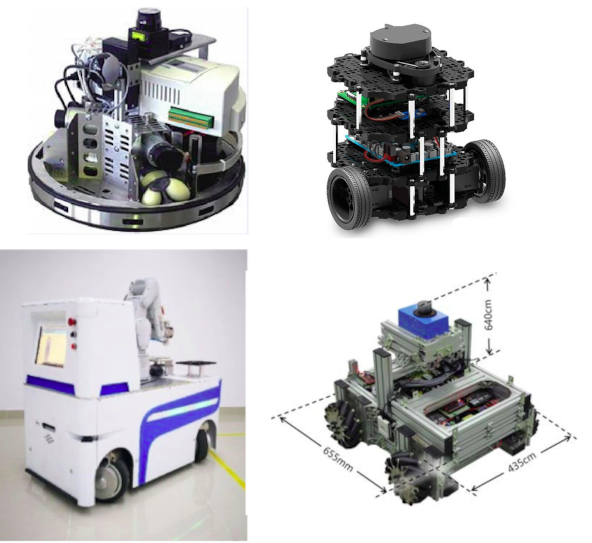
\includegraphics[trim=0 0 0 0,clip,width=0.5\textwidth]{Figs/Robot_types.png}
    \caption{Different types of robots}
    \label{fig:Aruco_bits}
\end{figure}


\subsection{Obstacle avoidance}
An important part for our mobile robot is the obstacle avoidance because it have to be able to response to the different situations that can affect its behaviour, In \citep{azeta2019obstacle}, they implemented the system using micro-controller Arduino Uno, a Wi-Fi module, an Arduino motor shield driver which controls the robot through the geared motors. The language that they used was C++ and the sensor was HC-SR04 ultrasonic sensor, the sensor emits an ultrasonic pulse each 0.3s to detect any obstruction between 2 and 400cm, finally they powered supply was a 7.4V 2400mAh lithium polymer battery.

Sometimes is possible to combine behaviors like wall following and obstacle avoidance \citep{hacene2019fuzzy}, that allows to make a simpler design. The usual way to deal with the obstacle avoidance is to define first a safety distance and if any of the sensors detect a distance under that limit, the robot will switch from the main behavior to the obstacle avoidance behavior. The definition of rules based on which sensors have detected an obstacle \citep{tzou2009high} \citep{hacene2019fuzzy} can be a good option when no artificial intelligence or complex techniques are used for the avoidance although this may reduce the efficiency to complete the main task.

Continuing with Obstacle avoidance in \citep{arcos2019optimal} presented another way to avoid an obstacle this way consists of use a time polynomial function to define the obstacle´s position, the method was used to satisfy such constraint computes the euclidean distance between the center of the robot and the center of the obstacle. That difference must to be bigger than a safe distance determined by the radius of the robot and the obstacle plus a security factor.

\subsection{Speed control}
The next step for the mobile robot was its movement for this we knew that we had to use control techniques to control the robot´s speed this is how we found this document \citep{abril2012analisis} that talks about if it´s necessary implement a control on a line tracker robot, because of this they made a comparison between a line tracker robot with fuzzy control that is a control technique that allows to work with information that is not accurate and the same robot but with a classic control. At the end of the document they conclude that with fuzzy control the mobile robot Robotino follows the desired trajectory receiving controller speeds up over 250m/s until 750m/s, on the other hand with the classic control the mobile robot Robotino can complete the desired trajectory but just with low speeds in addition we find another document that talks about the speed control with a PID controller, in \citep{thanh2019restaurant} they did a restaurant serving robot using double line-sensors following approach in combination with PID controller for stable speed outcome, the mobile robot is programmed to go to a specific table by mapping data and come back when it´s completed the task.Based on the line reading algorithm from two LED array line sensors implemented on micro controller.

\subsection{Location system}
Another thing to take in account its the location system because we need the real position of the robot to calculate the errors for the control that´s why we search how can we get the pose and position of the robot and we found this\citep{yuan2016rgb} where they did a location system with an Extend Kalman Filter(EKF) method to calculate robot position and pose also in \citep{tzou2009high} they made a location system using laser positioning system. The laser positioning system is used for rapid and precise positioning and guidance of the mobile robot. In other matters we found this document \citep{oltean2010position} that talks about a mobile robot that use 3 RFID readers with 13.56 MHz frequency are on the bottom of the robot and detect the RFID tags that are in the range of magnetic field of three RFID readers the RFID readers will obtain the absolute coordinates stored in the RFID tag and that´s how the robot reach the tables.The size of the RFID reader antenna
is 2.2 2.2 × cm and the size of the tag is 2.8 2.8 × cm.




\section{Fiducial markers}



\subsection{ArUco markers}
ArUco markers are very used for pose estimation and to implement automatic follow-up, for example, in the study of \citep{bacik2017autonomous} where ArUco markers are used for the navigation of a quadrocopter to make it follow a desired trajectory without any additional sensor, just using ArUco markers, in addition, they used ROS (Robotic Operating System), the open source software which is used for the mapping algorithms in that case. In \citep{jimenez2018sistema} we can see another application, in this case the cameras are static and the objective is to follow a object in the range vision of the cameras, the ArUco marker is used as a reference point for the pose estimation, which is cooperative, so it's necessary to combine the information of the two cameras to get better results. The fact that the cameras are statics is a problem when the object moves far away from the range vision, it's really important to have that in consideration as well as the issues that can generate the lighting changes in the environment at the moment of the detection. 

The resolution of the cameras didn't mean a significant change in the results of the detection as is concluded in \citep{kalaitzakis2021fiducial}, while things like contrast, white balance and images produced with smoother edges can decrease the accuracy and precision of the detection. ArUco had similar results in therms of detection rate compared with other fiducial markers like STag, AprilTag and ARTag, requires less hardware resources, so it’s implementation can be cheaper, it had really good results but it’s sensitive to small markers size and larger distances as is mentioned too in \citep{ferrao2018detection}.     


 
 
 
 
In the next table you can find some aplications directly related with our thesis:


\begin{table}[h!]
\caption{Direct applications}
\begin{centering}
\begin{tabular}{>{\centering}p{7cm}>{\centering}p{4cm}}
\hline 
\raggedright{}Description & \raggedright{}Reference\tabularnewline
\hline 
\raggedright{Implemetation of a waiter robot on a Pioneer 3DX robot} & \raggedright{}\citep{escudero2012robot}\tabularnewline
\hline 
\raggedright{}Mapping and location with a depth camera and movement base with gyroscope and odometry & \raggedright{}\citep{zhang2016approach}\tabularnewline
\hline 
\raggedright{}PID controller for stable speed and double-line sensor& \raggedright{}\citep{thanh2019restaurant}\tabularnewline
\hline 
\raggedright{}Reinforcement Q-learning PID Controller for a Restaurant Mobile Robot with Double Line-Sensors & \raggedright{}\citep{thanh2020reinforcement}\tabularnewline
\hline 
\raggedright{}Fuzzy Logic Based Control for Autonomous Mobile Robot Navigation& \raggedright{}\citep{omrane2016fuzzy}\tabularnewline
\hline 
\raggedright{}2 types of robots one to take the order and another to recive the dishes & \raggedright{}\citep{eksiri2015restaurant}\tabularnewline
\hline 
\end{tabular}
\par\end{centering}
\end{table}
\newpage

The implementation of the mobile robots affect positively the efficiency of a restaurant and also mitigate some charges that would have a human. We can see in this surveys the problems that present a normal restaurant.


In the study of \citep{florez2011factores} you can see surveys conducted about sanitation problems in some restaurants, some of those problems are simultaneous handling of money and food (17\%), wearing jewlery (15,2\%),Long fingernails (8,9\%) inter alia. On the other hand in \citep{armendariz2012riesgos} they talk about the health problems of workers also they carried out surveys with these results:

\begin{itemize}
\item 100\% of the waiters expressed high level concentration and physical efforts.
\item 87\% expressed forced work postures.
 
\item 80\% expressed that heavy handling is a risk in their professions.

\end{itemize}


 
 
\section{ROS} 
 ROS is a middleware that allows to control robots and make simulations quite close to the reality, it have been used most frequently in the recent years but it can be explored more, in \citep{osio2018desenvolupament} and \citep{zhang2020robot} are presented applications to real mobile robots through ROS where is remarkable the possibility of send commands to the robot using the local network and the easy integration of the computer vision with ROS. Another field of robotics where the use of ROS can be found is in the control of industrial arms as is presented in \citep{arents2018integration} where they integrate computer vision, artificial intelligence and the software Move It!, and as is mentioned there are ROS libraries, drivers and tools created for interfacing with industrial robots that prove the importance of ROS and how it can make the robot programming an easier task.
 
 


\cleardoublepage
\chapter{Conceptual frame/Main part}
\section{Estimation of the ArUco POSE}
\subsection{ArUco markers}
ArUco is a really useful open source library for marker detection through computer vision techniques, it contains some dictionaries with a large number of markers, where each marker can be identified with an unique id obtained from the recognition of a binary pattern in the markers as is shown in \autoref{fig:Aruco_bits} this patterns depends on the amount of bits according to the selected dictionary \citep{salinas2019aruco}.

\begin{figure}[h!]
    \centering
 	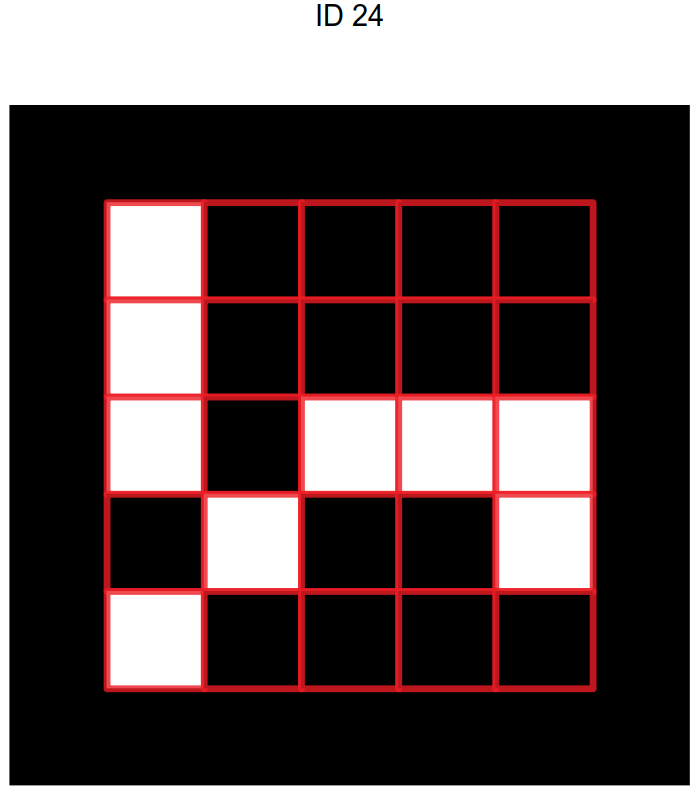
\includegraphics[trim=0 0 0 0,clip,width=0.4\textwidth]{Figs/ArUco24.png}
    \caption{ArUco marker from the original ArUco dictionary, which have a 5x5 bits dimensions}
    \label{fig:Aruco_bits}
\end{figure}

The wide number of marker id's and the accuracy in the detection of the Aruco markers and the fact that the library is available for Python makes it really appropriated to be used in this thesis work for the detection of each table. In the \autoref{fig:Aruco_detect}  we can see an example of the ArUco marker detection with Python and the Opencv library.

\begin{figure}[H]
    \centering
 	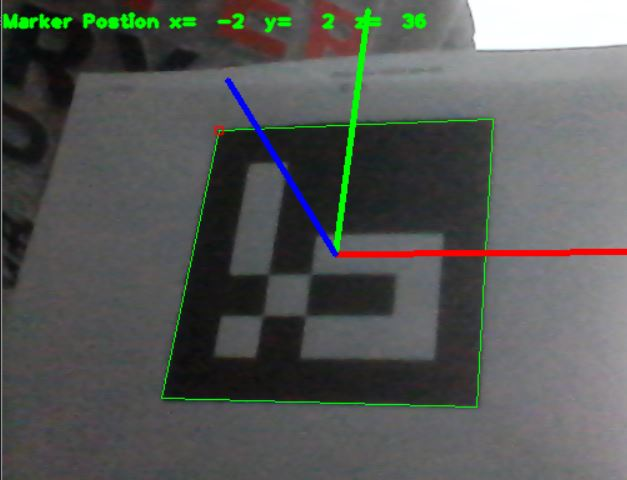
\includegraphics[trim=0 0 0 0,clip,width=0.6\textwidth]{Figs/Aruco.JPG}
    \caption{Marker position estimation}
    \label{fig:Aruco_detect}
\end{figure}

\subsection{Camera calibration}

The coordinates shown in \autoref{fig:Aruco_detect}, represents the estimated position of the marker respect to a frame located in the center of the camera, to get good results in the estimation is necessary to obtain the calibration and distortion matrix of the camera, there are two main ways to make the calibration process, the first one is with the ArUco calibration board, and the second one is with the classical Opencv chessboard which is the easier one and the selected in this case, in the \autoref{fig:Chessboard} we can see a set of pictures took with the camera, then this pictures are loaded to a Python program that select the good pictures and outputs the calibration and distortion matrix.

\begin{figure}[h!]
    \centering
 	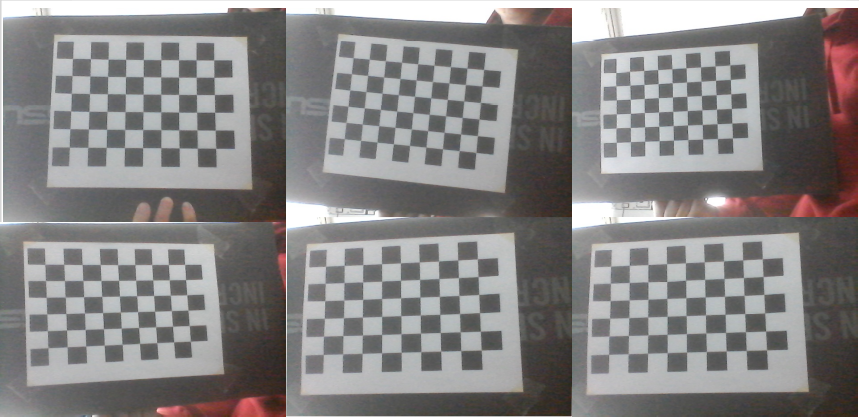
\includegraphics[trim=0 0 0 0,clip,width=0.6\textwidth]{Figs/Calib.png}
    \caption{Images for the camera calibration process}
    \label{fig:Chessboard}
\end{figure}



\section{Control design}
\subsection{Differential drive robot}
A differential drive robot consists in a robot with two motors attached to each wheel, this make possible to turn the robot but it can't move in any direction at any moment, it have to turn first. The robot can be represented in a kinematic form as a point moving in the space, this is known as the unicycle model, which translational and angular velocities are defined by:
\begin{equation}
    \dot{x}=v*cos(\theta)
\label{eq:X_dot}
\end{equation}
\begin{equation}
    \dot{y}=v*sin(\theta)
\label{eq:Y_dot}
\end{equation}
\begin{equation}
    \dot{\theta}=\omega
\label{eq:Omega}
\end{equation}


Where $v$ and $\omega$ are derivated from the followings equations, R is the radius of the wheels, L is the separation between the wheels, $v_{r}$ and $v_{l}$ are the velocities of each wheel in rad/s:
\[v=\frac{R}{2}*(v_r+v_l)\]
\[\omega=\frac{R}{L}*(v_r-v_l)\]
Replacing $v$ and $\omega$ in \autoref{eq:X_dot}, \autoref{eq:Y_dot} and \autoref{eq:Omega}:
\[\dot{x}=\frac{R}{2}*(v_r+v_l)*cos(\theta)\]
\[\dot{y}=\frac{R}{2}*(v_r+v_l)*sin(\theta)\]
\[\dot{\phi}=\frac{R}{L}*(v_r-v_l)\]





\subsection{Go-to-goal behavior}

First we need to define the errors of position and orientation from the robot to the goal:

\[e_x=X_d-X\]
\[e_y=Y_d-Y\]
\[e_{heading}=\theta_d-\theta\]


\[V=K_{pv}*\sqrt{e_x^2+e_y^2}\]
\[\omega=K_{p\omega}*\arctan{\frac{\sin{e_{heading}}}{\cos{e_{heading}}}}\]




\subsection{Obstacle avoidance}


\begin{figure}[h!]
    \centering
 	\includegraphics[trim=0 0 0 0,clip,width=0.6\textwidth]{Figs/Flowchart.eps}
    \caption{Fluid process diagram}
    \label{fig:Chessboard}
\end{figure}

\section{ROS and Gazebo simulation}
\subsection{ROS}
The Robot Operating System (ROS) is an open-source framework that helps researchers and developers build and reuse code between robotics applications. ROS is also a global open-source community of engineers, developers and hobbyists who contribute to making robots better, more accessible and available to everyone.
\subsubsection{Topics}
Topics are named buses over which nodes exchange messages. Topics have anonymous publish/subscribe semantics, which decouples the production of information from its consumption. In general, nodes are not aware of who they are communicating with. Instead, nodes that are interested in data subscribe to the relevant topic; nodes that generate data publish to the relevant topic. There can be multiple publishers and subscribers to a topic.
\subsubsection{Nodes}
A node is a process that performs computation. Nodes are combined together into a graph and communicate with one another using streaming topics, RPC services, and the Parameter Server. These nodes are meant to operate at a fine-grained scale; a robot control system will usually comprise many nodes. For example, one node controls a laser range-finder, one Node controls the robot's wheel motors, one node performs localization, one node performs path planning, one node provides a graphical view of the system, and so on.
\subsection{Gazebo}
\subsection{Simulated environment}
\subsubsection{URDF}
An URDF model is a XML-based representation of the physics and the visual properties of the robot and the other world elements, this model is necessary for the simulation 
\begin{figure}[h!]
    \centering
 	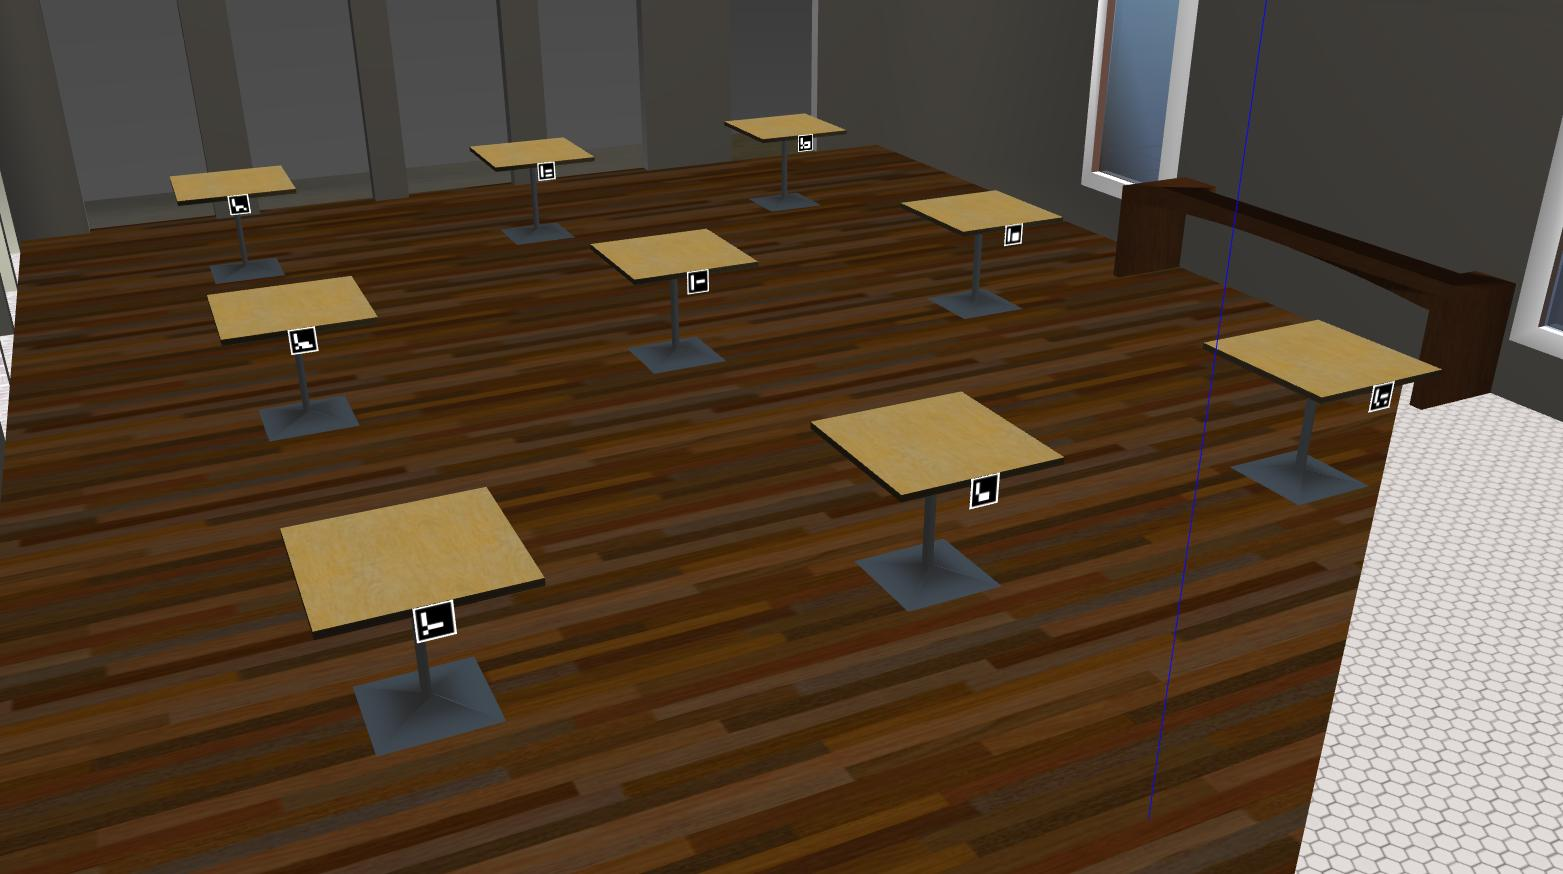
\includegraphics[trim=0 0 0 0,clip,width=0.8\textwidth]{Figs/Gzworld.jpg}
    \caption{Simulated tables and it's ArUco markers attached to each one in a Gazebo world}
    \label{fig:Gzworld}
\end{figure}
\begin{figure}[h!]
    \centering
 	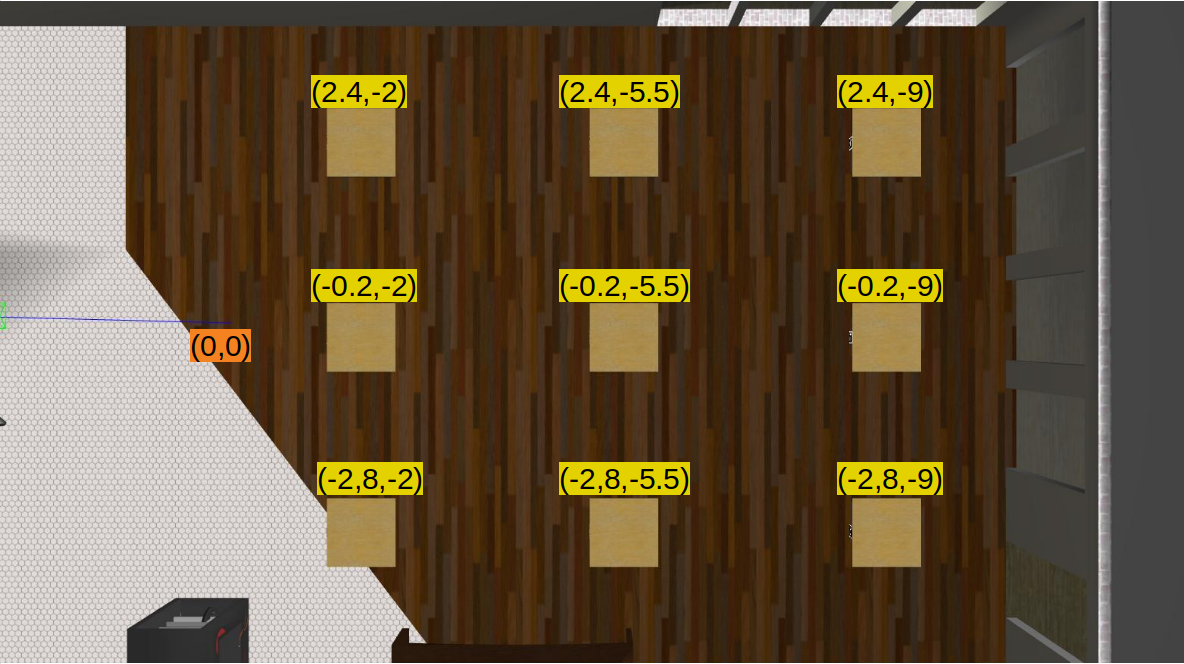
\includegraphics[trim=0 0 0 0,clip,width=0.8\textwidth]{Figs/Cords_tables.png}
    \caption{Coordinates of the tables in the simulated environment}
    \label{fig:Cords_Tables}
\end{figure}

In the simulated world the robot follows a predefined trajectory when no ArUco marker is detected, the robot navigates through the simulated restaurant trying to find the requested ArUco marker and when it finally detects it switch to a go to the table behavior.

\begin{figure}[h!]
    \centering
 	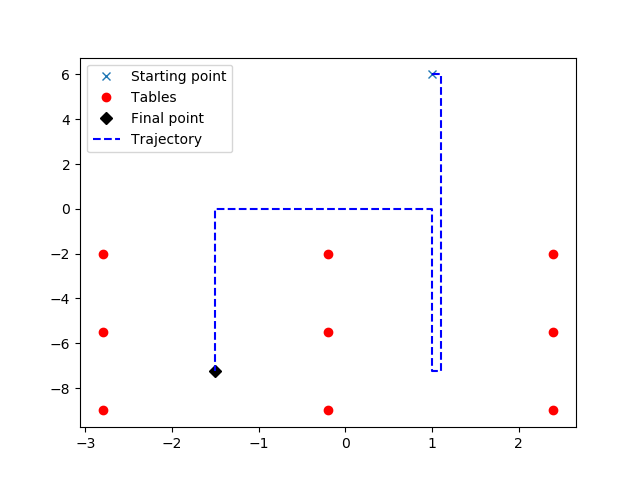
\includegraphics[trim=0 0 0 0,clip,width=0.8\textwidth]{Figs/Trajectory1.png}
    \caption{Predefined trajectory}
    \label{fig:Cords_Tables}
\end{figure}


\newpage
\section{Prototype design}
The hardware design of our mobile robot was based on Turtlebot3 Burger  it´s a mobile robot designed by Robotics company, The Turtlebot3 Burger its a modular and customisable mobile robot which components are a RaspberryPi 3, Laser Distance sensor, OpenCR and Dynamixel X.

\begin{figure}[h!]
    \centering
 	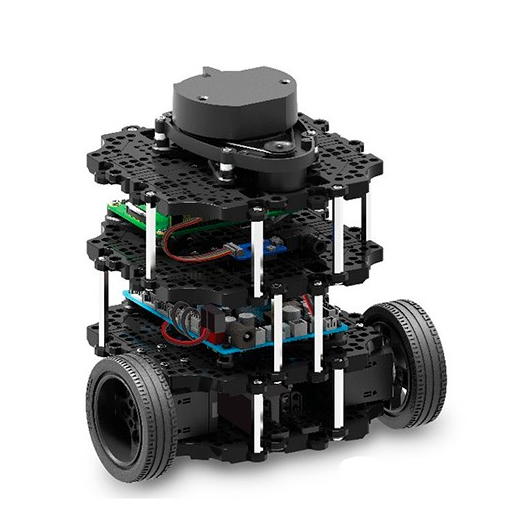
\includegraphics[trim=0 0 0 0,clip,width=0.3\textwidth]{Figs/Burger.png}
    \caption{TurtleBot 3 Burger}
    \label{fig:Burger}
\end{figure}

Our mobile robot was designed on Autodesk Inventor software and then 3D printed, the base material is PLA that is a plant-based, biodegradable plastic and the material of the columns is Aluminum.

The parts of our design are 3 bases supported by 4 columns each one, the first has 15 cm radius and 1 cm thick, the second base has 15 cm radius and 0.5 cm thick and the second has 10 cm radius and 0.5 cm thick, the columns have 5mm radius and 30cm in length, the robot´s hardware are as follows. The Raspberry Pi, Li-po Batteries, H-bridges and ultrasonic sensors are on the first base and the camera is on the top of the mobile robot in addition the motors and the encoder are bracket mounted on the bottom of the base.    

\begin{figure}[h!]
    \centering
 	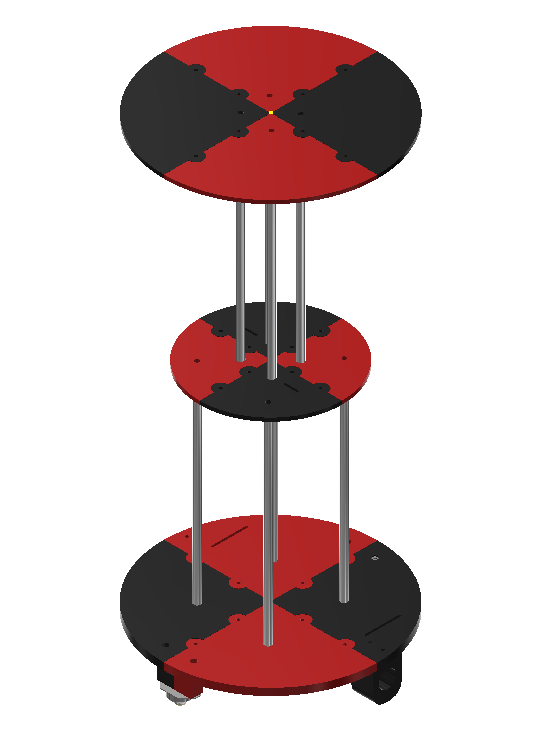
\includegraphics[trim=0 0 0 0,clip,width=0.45\textwidth]{Figs/Robot.png}
    \caption{Mobile Robot design on Autodesk Inventor}
    \label{fig:Robot}
\end{figure}

\newpage
\section{Implementation}

\subsection{Raspberry Pi 3}
The Raspberry Pi is a single-board computer commonly used in robotics and IoT applications, due to the fact that ROS can be run in the Raspberry, makes it appropriated to be selected as the main component of the project, here is where the ROS topics with the information of the sensor will be published, and through it the commands to move the robot will be sent.

\begin{figure}[h!]
    \centering
 	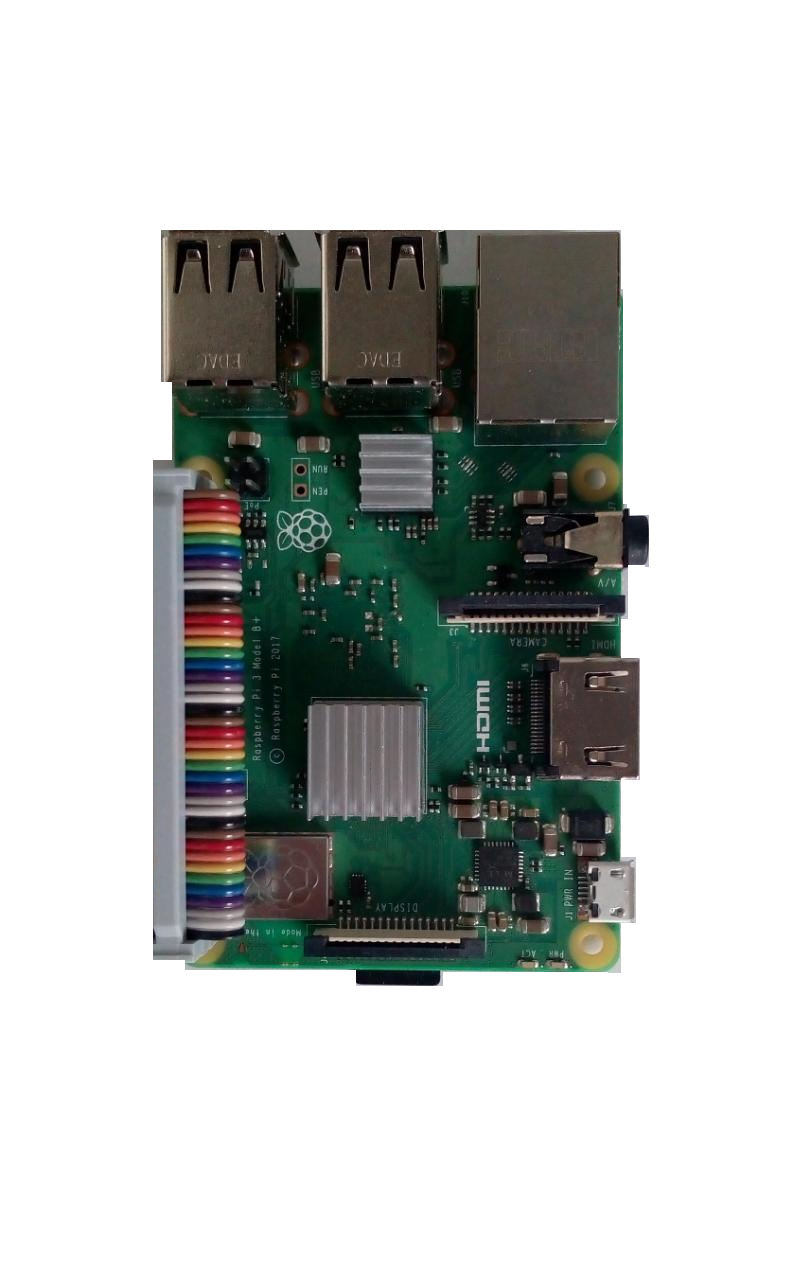
\includegraphics[trim=0 0 0 0,clip,width=0.4\textwidth]{Figs/Raspberry1.png}
    \caption{Raspberry Pi Model B+}
    \label{fig:RPI}
\end{figure}

\begin{figure}[H]
    \centering
 	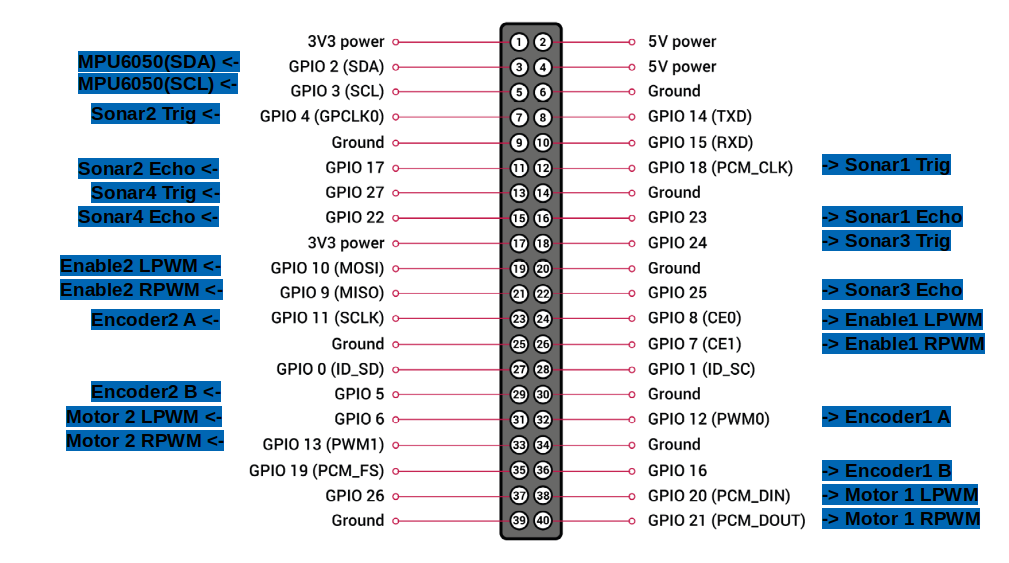
\includegraphics[trim=0 0 0 0,clip,width=0.8\textwidth]{Figs/RPI.png}
    \caption{Raspberry Pi GPIO ports connection}
    \label{fig:RPI_ports}
\end{figure}

\begin{table}[H]
\caption{Raspberry Pi B+ specifications}
\begin{centering}
\begin{tabular}{>{\centering}p{7cm}>{\centering}p{4cm}}
\hline 
\raggedright{}Power supply & \raggedright{}5V/2.5A DC\tabularnewline
\hline 
\raggedright{}SoC & \raggedright{}Broadcom BCM2837\tabularnewline
\hline 
\raggedright{}CPU & \raggedright{}1.4GHz 64-bit quad-core ARMv8\tabularnewline
\hline 
\raggedright{}USB ports & \raggedright{}4\tabularnewline
\hline 
\raggedright{}GPIO ports & \raggedright{}40\tabularnewline
\hline 
\raggedright{}RAM & \raggedright{}1 GB\tabularnewline
\hline 
\raggedright{}Disk & \raggedright{}8 GB SD card\tabularnewline
\hline 
\raggedright{}OS & \raggedright{}Raspbian\tabularnewline
\hline 
\raggedright{}ROS distro & \raggedright{}Melodic\tabularnewline
\hline 
\end{tabular}
\par\end{centering}
\end{table}

\subsection{Ultrasonic sensor HC-SR04}
This sensor is used for distance measurement, the sensor have a transmitter and a receiver as is shown in  \autoref{fig:Sonar}, basically it generates a wave sound and then listen to the echo produced when the wave bounces in the object in front of the sensor, the time that the wave takes to go back to the sensor and the sound speed are used to calculate the distance between the sensor and the obstacle with the following equation \citep{morgan2014hcsr04}: 
\begin{equation}
    distance=speed*time
\label{eq:Distance}
\end{equation}
The trigger pin of the sensor receives is used to send a 10 nano seconds ultrasonic pulse, the echo pin sets to high while the pulse is being received, the time that echo pin is set to high ($t$), the distance traveled to the object and the distance traveled back to the sensor ($2d$) and the sound speed $(340 m/s)$ are replaced in \autoref{eq:Distance}, obtaining:
\[2d=340m/s*t\]
\[d=170m/s*t\]
\begin{figure}[h!]
    \centering
 	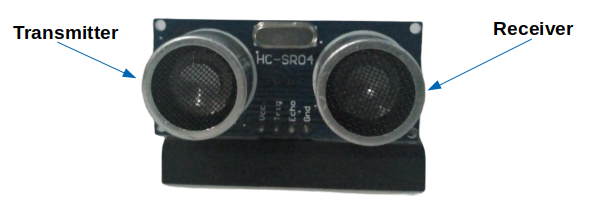
\includegraphics[trim=0 0 0 0,clip,width=0.8\textwidth]{Figs/Sonar1.png}
    \caption{Sonar sensor}
    \label{fig:Sonar}
\end{figure}

\begin{table}[h!]
\caption{Hc-Sr04 specifications}
\begin{centering}
\begin{tabular}{>{\centering}p{7cm}>{\centering}p{4cm}}
\hline 
\raggedright{}Power supply & \raggedright{}+5V DC\tabularnewline
\hline 
\raggedright{}Effectual angle & \raggedright{}<15°\tabularnewline
\hline 
\raggedright{}Ranging distance & \raggedright{}2-400 cm\tabularnewline
\hline 
\raggedright{}Resolution & \raggedright{}0.3 cm\tabularnewline
\hline 
\raggedright{}Measuring angle & \raggedright{}30°\tabularnewline
\hline 
\end{tabular}
\par\end{centering}
\end{table}



\subsection{H-Bridge BTS-7960}

The H-Bridge BTS-7960 alloys to control the velocity of each motor, it’s able to support high current levels, what makes it ideal for control high-torque motors.
\begin{table}[H]
\caption{H-Bridge Bts7960 specifications}
\begin{centering}
\begin{tabular}{>{\centering}p{7cm}>{\centering}p{4cm}}
\hline 
\raggedright{}Power supply & \raggedright{}5.5-27 V\tabularnewline
\hline 
\raggedright{}Logic input voltage & \raggedright{}-0.3-5 V\tabularnewline
\hline 
\raggedright{}Max frequency operation & \raggedright{}25 KHz\tabularnewline
\hline 
\raggedright{}Max current supported & \raggedright{}43 A\tabularnewline
\hline 
\end{tabular}
\par\end{centering}
\end{table}


\begin{figure}[H]
    \centering
 	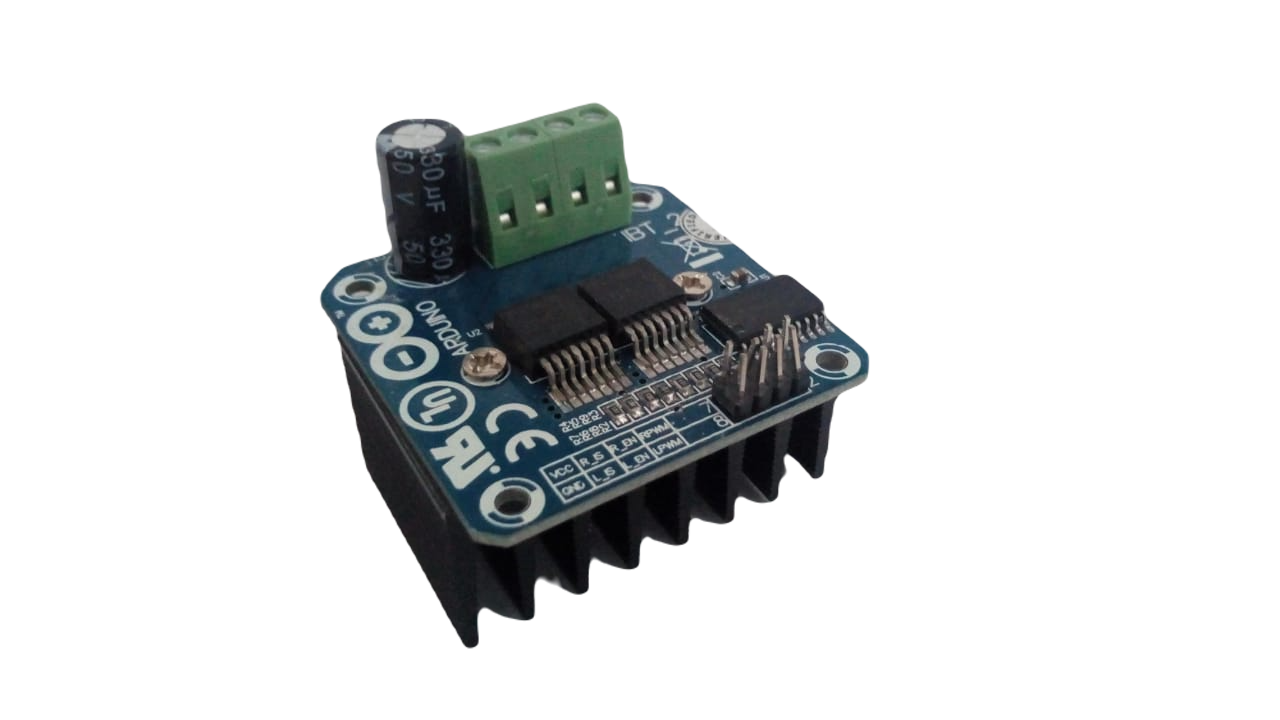
\includegraphics[trim=0 0 0 0,clip,width=0.6\textwidth]{Figs/Hbridge1.png}
    \caption{H-Bridge}
    \label{fig:H-bridge}
\end{figure}

\subsection{Generic Raspberry Pi camera PI REV 1.3}
The generic raspberry pi camera have a good resolution and it’s price is very low compared to other cameras with similar properties. It can be connected directly to the Raspberry Pi through a CSI interface.
\begin{figure}[H]
    \centering
 	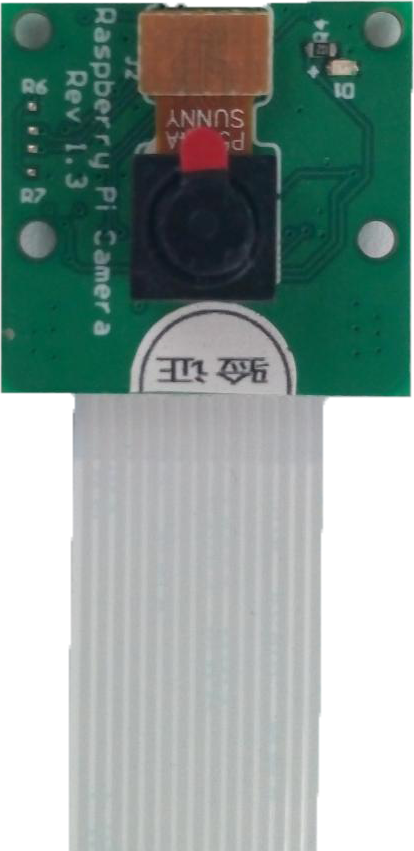
\includegraphics[trim=0 0 0 0,clip,width=0.2\textwidth]{Figs/Rasp_camera.png}
    \caption{Raspberry Pi camera PI REV 1.3}
    \label{fig:Rasp_camera}
\end{figure}

\begin{table}[H]
\caption{PI REV 1.3 specifications}
\begin{centering}
\begin{tabular}{>{\centering}p{7cm}>{\centering}p{4cm}}
\hline 
\raggedright{}Resolution & \raggedright{}5 MP\tabularnewline
\hline 
\raggedright{}Maximum static images size & \raggedright{}2592x1944\tabularnewline
\hline 
\raggedright{}Video formats & \raggedright{}1080p30, 720p60 and 640x480p60/90\tabularnewline
\hline 
\end{tabular}
\par\end{centering}
\end{table}

\subsection{Motors, encoders and batteries}

The selected motor is a JGA25-370 DC motor with a torque of 10 Kg-cm what makes it capable to move the robot even when it have a plate over it, this motor have attached to it a hall effect encoder which will be used for the measurement of the position and the velocity of the robot and the motors.  

\begin{figure}[H]
    \centering
 	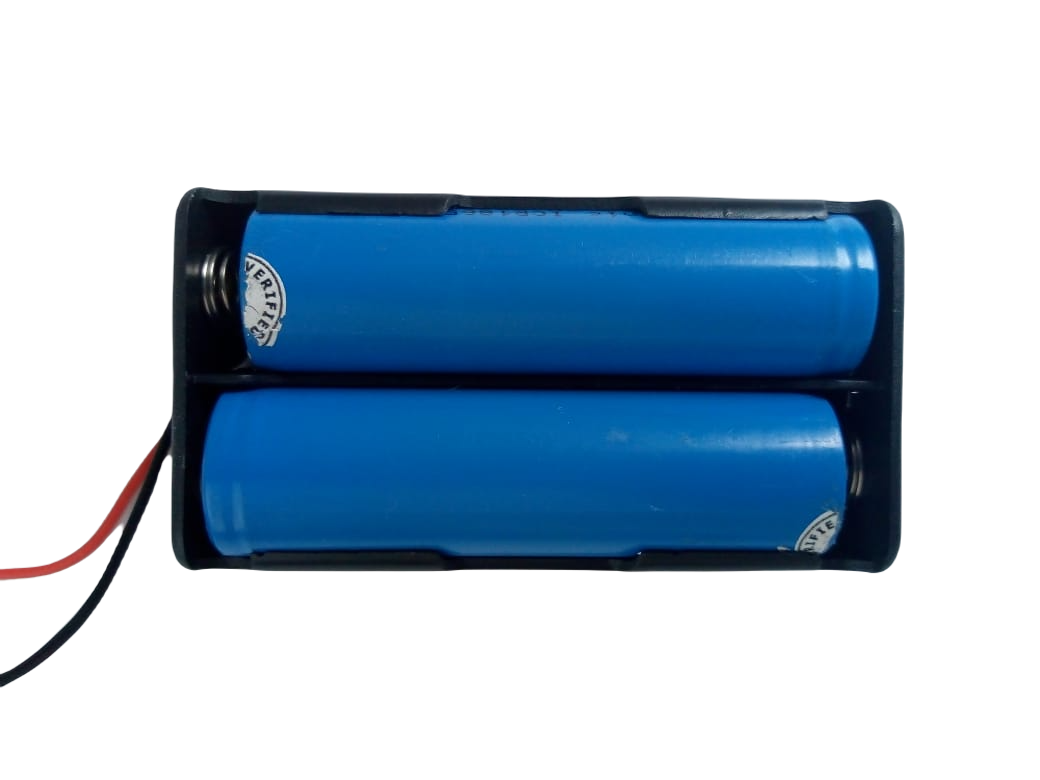
\includegraphics[trim=0 0 0 0,clip,width=0.4\textwidth]{Figs/Batteries1.png}
    \caption{18650 Batteries}
    \label{fig:Batteries}
\end{figure}

\begin{table}[H]
\caption{Parts specifications}
\begin{centering}
\begin{tabular}{>{\centering}p{7cm}>{\centering}p{4cm}}
\hline 
\raggedright{}Batteries & \raggedright{}3,7V, 2200 mAh\tabularnewline
\hline 
\raggedright{}Encoders resolution& \raggedright{}748 PPR\tabularnewline
\hline 
\raggedright{}Encoders supply voltage & \raggedright{}3-3,3V\tabularnewline
\hline 
\raggedright{}Motors supply voltage & \raggedright{}6V\tabularnewline
\hline 
\raggedright{}Velocity & \raggedright{}100 RPM\tabularnewline
\hline 
\end{tabular}
\par\end{centering}
\end{table}

\newpage
\section{Method}

Para la realización del proyecto se elige la metodología de investigación de la ruta crítica.
\begin{table}[h!]
\caption{Tabla para el análisis PERT}
\begin{centering}
\par\end{centering}
\begin{centering}
\begin{tabular}{l>{\raggedright}p{5cm}lllc}
\hline 
\textbf{ID} & \textbf{Actividad} & \textbf{a(semanas)} & \textbf{m(semanas)} & \textbf{b(semanas)} & \textbf{T}\tabularnewline
\hline 
\textbf{A} & Introducción a visión por computadora & 2 & 4 & 6 & 4\tabularnewline
\hline 
\textbf{B} & Recopilar información & 3 & 5 & 7 & 5\tabularnewline
\hline 
\textbf{C} & Organizar información & 2 & 4 & 6 & 4\tabularnewline
\hline 
\textbf{D} & Pruebas detección marcadores ArUco & 1 & 3 & 5 & 3\tabularnewline
\hline 
\textbf{E} & Introducción a entornos de simulación como Robotino view, Gazebo y
ROS & 4 & 5 & 7 & 5\tabularnewline
\hline 
\textbf{F} & Revisión de propuesta de anteproyecto y correcciones & 2 & 4 & 5 & 4\tabularnewline
\hline 
\textbf{G} & Control del Robotino y creación de técnicas para evasión de obstáculos & 6 & 9 & 13 & 9\tabularnewline
\hline 
\textbf{H} & Pruebas y correcciones & 2 & 4 & 5 & 4\tabularnewline
\hline 
\end{tabular}
\par\end{centering}
\centering{}
\end{table}

Donde $a$ es un tiempo optimista para la realización de la actividad, $m$ es un tiempo medio, $b$ es un tiempo pesimista y $T$ está dada por: 
\[T=\frac{(a+4m+b)}{6}\]
\newpage
\begin{table}[h!]
\caption{Tabla de actividades planificadas según la propuesta de investigación}
\begin{centering}
\begin{tabular}{l>{\raggedright}p{5cm}ll}
\hline 
\textbf{ID} & \textbf{Actividad} & \textbf{Actividad predecesora} & \textbf{Tiempo(Semanas)}\tabularnewline
\hline 
\textbf{A} & Introducción a visión por computadora & Ninguna  & 4\tabularnewline
\hline 
\textbf{B} & Recopilar información & A & 5\tabularnewline
\hline 
\textbf{C} & Organizar información & A-B & 4\tabularnewline
\hline 
\textbf{D} & Pruebas detección marcadores ArUco & A-B-C & 3\tabularnewline
\hline 
\textbf{E} & Introducción a entornos de simulación como Robotino view, Gazebo y
ROS & A-B-C-D & 5\tabularnewline
\hline 
\textbf{F} & Revisión de propuesta de anteproyecto y correcciones & A-B-C-D-E & 4\tabularnewline
\hline 
\textbf{G} & Control del Robotino y creación de técnicas para evasión de obstáculos & A-B-C-D-E-F & 9\tabularnewline
\hline 
\textbf{H} & Pruebas y correcciones & A-B-C-D-E-F-G & 4\tabularnewline
\hline 
\end{tabular}
\par\end{centering}
\end{table}

\begin{figure}[h!]
    \centering
    \resizebox*{14cm}{!}{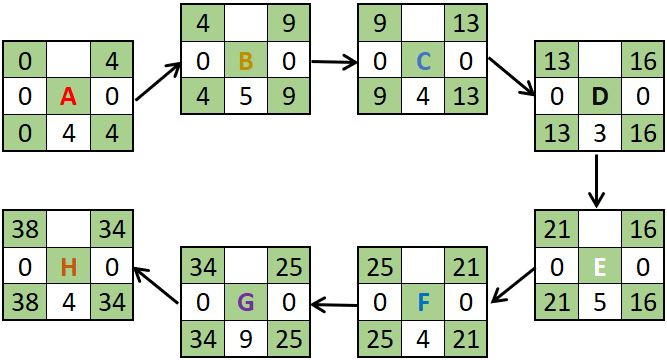
\includegraphics{Figs/RedAON2.JPG}}
    \caption{Diagrama PERT para el proyecto}
    \label{fig:PERT}
\end{figure}

\cleardoublepage
\chapter{Conclusion}





